\documentclass[openany]{book}
\usepackage{amsmath}
\usepackage{bm}
\usepackage{makeidx}
\usepackage{tikz}
\usetikzlibrary{arrows.meta}
\usepackage[
  top=1.25in,
  bottom=1.25in,
  left=1.25in,
  right=1.25in,
  bindingoffset=0.25in,
  heightrounded,
]{geometry}

\def\lsqb{\left[}
\def\rsqb{\right]}
\def\sqb#1{\lsqb #1 \rsqb}
\def\xsig{x\sqb{n}}

\makeindex
\begin{document}
\title{The DSP Cookbook}
\date{October 2017}
\author{Pelle Juul Christensen}
\maketitle
\tableofcontents

\chapter{Theory}
\section{Sine Wave}
\index{Sine waves}
\index{Sin}
\index{Cos}
Sine waves are waves generated by the functions $\sin$ and $\cos$. Given a variable $t$ we go $t$ radians along the unit circle \footnote{A unit circle is simply a circle with a radius of 1}. The point at $t$ radians will have coordinates $(\cos(t), \sin(t))$ --- $\cos(t)$ is the projection of the point onto the x-axis, $\sin(t)$ is the projection onto the y-axis.



\begin{figure}[h]
\centering
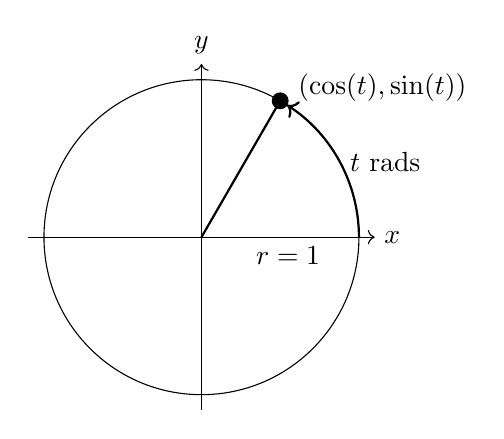
\begin{tikzpicture}[scale=2, domain=0:3]
    \draw (0, 0) circle [radius=1.0];
    \draw [->] (-1.1, 0) -- (1.1, 0) node [right] {$x$} node[pos=0.75, below] {$r=1$};
    \draw [->] (0, -1.1) -- (0, 1.1) node [above] {$y$};
    \draw[thick] (0, 0) -- (60:1) node[pos=1.1, right] {$(\cos(t), \sin(t))$};
    \filldraw (60:1) circle [radius=0.05];
    \draw[thick] [->] (1, 0) arc (0:57:1) node[pos=0.5,right] {$t$ rads};
\end{tikzpicture}
\end{figure}

\index{period}
Sinusoids have a period of $2 \pi$ (a full arc), thus if we multiply $t$ by $2\pi$ to get $\sin(2 \pi t)$, we will get a period of $1$. If $t$ is time in seconds, we will have one period per second.

To get more or less periods per second we multiply $t$ by that amount. For example $\sin(2 \pi t 440)$ has 440 periods per second.

\index{Frequency}
\index{Hertz}
\index{Hz|see {Hertz}}
Periods per second is measured in $Hertz$ which has the unit $1/s$, which is also called the frequency of a wave. To calculate the period of a sine wave at a specific frequency $f$, you use $1/f$, e.g. a sine wave at $440Hz$ will have a period of $1/f=0.002s$. So the general equation for a sine wave at a specific frequency is

\begin{equation}
    \sin(2\pi tf)
\end{equation}

\section{Causal Systems}
In systems with memory, we need to agree on what should happen when $n < 0$. Usually we will use $x\left[n\right] = 0 \text{ for } n < 0$. Such a system is said to be \textit{cusal}.

If we have a system where $x\left[n\right] \neq 0 \text{ for } n < 0$, then the system is said to be \textit{non-causal}.

\section{Difference Equations}
The general form of a difference equation is

\begin{equation}
\begin{split}
    y\sqb{n} = a_1 y\sqb{n - 1} + a_2 y\sqb{n-2} + \dots + a_N y\sqb{n-N} + \\
        b_0 x\sqb{n} + b_1 x\sqb{n - 1} + b_2 x\sqb{n - 2} + \dots + b_L\sqb{n - L}.
\end{split}
\end{equation}

Also written as

\begin{equation}
    y\sqb{n} = \sum_{k=1}^N a_k y\sqb{n - k} + \sum_{k=0}^L b_k x\sqb{n - k}.
\end{equation}

Where the $y\sqb{\cdot}$ components determine the recursive (feedback) characteristic, and the $x\sqb{\cdot}$ components the non-recursive characteristic.

\section{Linear Time-Invariant System}
\index{Linear Time-Invariant System}
\index{LTI|see {Linear Time-Invariant System}}

A system $T(x\sqb{n})$ is \textit{linear time-invariant} (LTI) is it is both linear and time-invariant.

A system is linear if it supports the scalability property \index{Linearity property}
\begin{equation}
    T(\alpha \xsig) = \alpha T(\xsig).
\end{equation}
As well as the superposition property \index{Superposition property}
\begin{gather}
    T(x_3\sqb{n}) = T(x_1\sqb{n} + x_2\sqb{n}) =  T(x_1\sqb{n}) + T(x_2\sqb{n}), 
\end{gather}
where $x_3\sqb{n} = x_1\sqb{n} + x_2\sqb{n}$.

A system is time-invariant if it meets the condition
\index{Time-invariant}
\begin{equation}
    x\sqb{n - L} = y\sqb{n - L}
\end{equation}
for some delay $L$ --- a delay in the input signal will cause a corresponding delay in the output signal.

A system is LTI if all of its subcomponents are LTIs.

\section{Impulse Response}
\index{Impulse response}
An impulse is a short spike in amplitude. The ideal impulse signal is defined by

\begin{equation}
    \delta\sqb{n} =
        \begin{cases}
            1, & \text{if } n = 0 \\
            0, & \text{otherwise}
        \end{cases}.
\end{equation}

The \textit{impulse response} of a system is how it reacts to an input of $\xsig = \delta\sqb{n}$. In this
case the ouput of the system is normally denoted $h\sqb{n}$.

LTI systems can be described completely by their impulse responses. To obtain the output of a system based on an impulse response, one should convolute the input signal with the impulse response
\begin{equation}
    T(\xsig) = \xsig * h_T\sqb{n}.
\end{equation}

\index{Finite impulse repsonse}
\index{FIR|see {Finite impulse repsonse}}
A system has \textit{finite impulse response} (FIR) if it does not contain any recursive components. In that case the impulse response is determined by
\begin{equation}
    h\sqb{n} = T(\delta\sqb{n}) = \sum_{k = 0}^L b_k \delta\sqb{n - k}.
\end{equation}
The impulse response of FIR systems will always converge to zero.

\index{Infinte impulse response}
\index{IIR|see {Infinte impulse response}}
A system has \textit{infinte impulse reponse} (IIR) if it contains recursive components. In that case the impulse response is determined by
\begin{equation}
    h\sqb{n} = T(\delta\sqb{n}) = \sum_{k=1}^N a_k h\sqb{n - k} + \sum_{k = 0}^L b_k \delta\sqb{n - k}.
\end{equation}
\index{Stability}
\index{Stable}
\index{Unstable}
Some IIR systems will converge to a state of near-zero. Such systems are said to be \textit{stable}. IIR systems can also be \textit{unstable}, which means that their output will be non-convergent (i.e. blow up).

\section{Convolution}
\index{Convolution}
The \textit{convolution} of two signals $\xsig$ and $h\sqb{n}$ is defined as
\begin{equation}
    \xsig * h\sqb{n} = \sum_{m = -\infty}^{m = \infty} x\sqb{n - m}h\sqb{m}.
\end{equation}

In reality $m$ will be bounded by the sizes of the signals. If $\xsig$ has size $N$ and $h\sqb{n}$ size $M$, then $m$ should be within $0$ and $M$, since no samples is defined before $0$, and no smaples in $h\sqb{x}$ are defined after $M$. The equation is then
\begin{equation}
    \xsig * h\sqb{n} = \sum_{m = 0}^{M} x\sqb{n - m}h\sqb{m}.
\end{equation}
The result will be defined for $n$ in $0 \leq n < N + M$.

Convolution is commutative, meaning that
\begin{equation}
    \xsig * h\sqb{n} = h\sqb{n} * \xsig.
\end{equation}
It is also associative, which means that
\begin{equation}
    g\sqb{x} * (\xsig * h\sqb{n}) = (g\sqb{x} * \xsig) * h\sqb{n},
\end{equation}
as well as distributive
\begin{equation}
    g\sqb{x} * (\xsig + h\sqb{n}) = (g\sqb{x} * \xsig) + (g\sqb{x} *  h\sqb{n}).
\end{equation}

\section{Frequency Response}
\index{Frequency response}
\index{Bode diagram}
The frequency response of a system describes how it responds to signals of a specific frequency, in terms of magnitude and phase. The frequency response of a system is usually shown as a plot with frequency on the x-axis and amplitude on the y-axis. If the plot is presented with a logarithmic frequency scale, it is sometimes called a *Bode* diagram.


\printindex

\end{document}
